% Cover 5 v2: "Spectrum Flow" — refined, professional
\documentclass[tikz,border=0mm]{standalone}
\usepackage{tikz}
\usetikzlibrary{calc}
\usepackage{xcolor}
\usepackage[T1]{fontenc}

\definecolor{deeppurple}{RGB}{22,6,50}
\definecolor{paneldark}{RGB}{15,4,36}
\definecolor{tealdeep}{RGB}{0,78,90}
\definecolor{tealbright}{RGB}{65,215,195}
\definecolor{tealaccent}{RGB}{110,235,218}
\definecolor{lavender}{RGB}{172,132,215}
\definecolor{lavlight}{RGB}{205,178,238}
\definecolor{peach}{RGB}{238,148,85}
\definecolor{peachlight}{RGB}{252,190,140}
\definecolor{whitesoft}{RGB}{244,241,255}
\definecolor{whitedim}{RGB}{190,185,210}

\begin{document}
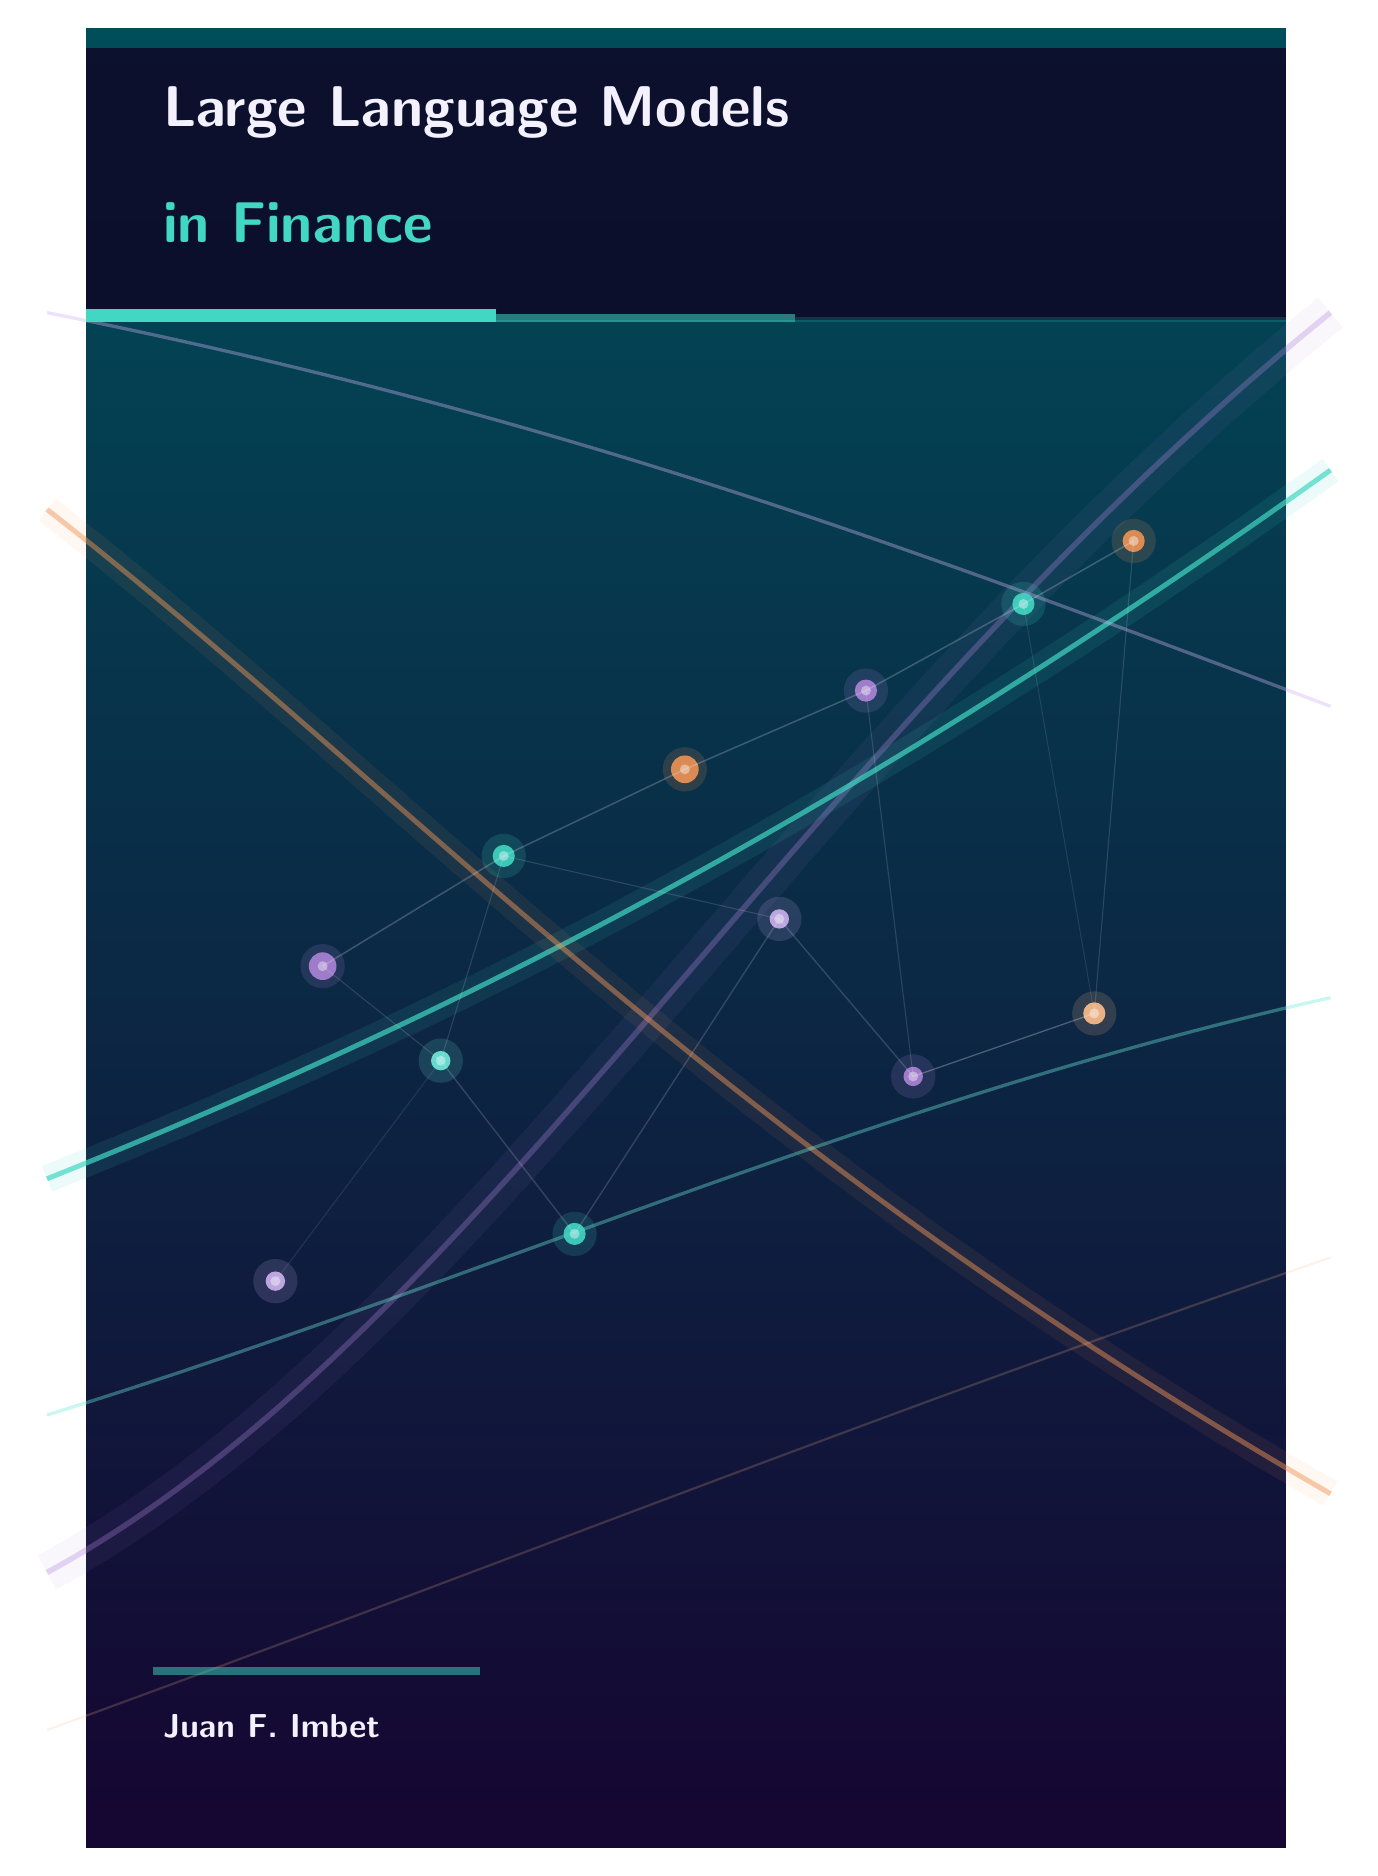
\begin{tikzpicture}

  % ── GRADIENT BACKGROUND ────────────────────────────────────────────────────
  % bottom = deep purple, top = teal-dark; gentle 0.15-step bands
  \foreach \y in {0,0.15,...,23.0}{
    \pgfmathsetmacro{\t}{\y/22.86}
    \pgfmathsetmacro{\r}{int(22 + (0-22)*\t)}
    \pgfmathsetmacro{\g}{int(6  + (78-6)*\t)}
    \pgfmathsetmacro{\b}{int(50 + (90-50)*\t)}
    \definecolor{bkg}{RGB}{\r,\g,\b}
    \fill[bkg] (0,\y) rectangle (15.24,\y+0.17);
  }

  % ── FLOWING BEZIER STREAMS ─────────────────────────────────────────────────
  % Each stream: wide soft glow  +  sharp bright line

  % S1 — lavender: sweeps low-left to upper-right
  \draw[lavender,line width=14pt,opacity=0.07]
    (-0.5,3.5) .. controls (5,6.5) and (9,14) .. (15.8,19.5);
  \draw[lavender,line width=2pt,opacity=0.32]
    (-0.5,3.5) .. controls (5,6.5) and (9,14) .. (15.8,19.5);

  % S2 — tealbright: gentle upward arc (primary line)
  \draw[tealbright,line width=10pt,opacity=0.10]
    (-0.5,8.5) .. controls (4.5,10.5) and (9.5,13) .. (15.8,17.5);
  \draw[tealbright,line width=1.8pt,opacity=0.70]
    (-0.5,8.5) .. controls (4.5,10.5) and (9.5,13) .. (15.8,17.5);

  % S3 — peach: diagonal descent (crosses S1 & S2)
  \draw[peach,line width=10pt,opacity=0.08]
    (-0.5,17) .. controls (4,13.5) and (8,9) .. (15.8,4.5);
  \draw[peach,line width=1.8pt,opacity=0.48]
    (-0.5,17) .. controls (4,13.5) and (8,9) .. (15.8,4.5);

  % S4 — lavlight: shallower arc (upper zone)
  \draw[lavlight,line width=1.2pt,opacity=0.38]
    (-0.5,19.5) .. controls (6,18.2) and (10.5,16.5) .. (15.8,14.5);

  % S5 — tealaccent: lower arc
  \draw[tealaccent,line width=1.2pt,opacity=0.38]
    (-0.5,5.5) .. controls (5,7.2) and (10,9.5) .. (15.8,10.8);

  % S6 — peachlight: subtle bottom trace
  \draw[peachlight,line width=0.8pt,opacity=0.20]
    (-0.5,1.5) .. controls (5,3.5) and (10,5.5) .. (15.8,7.5);

  % ── NETWORK NODES ─────────────────────────────────────────────────────────
  % Uniform sizing (3–5pt), all warm tones, outer glow + white highlight
  % Nodes: glow + filled dot + highlight
  \newcommand{\netnode}[4]{%
    \fill[#4,opacity=0.16] (#1,#2) circle (8pt);
    \fill[#4,opacity=0.90] (#1,#2) circle (#3);
    \fill[white,opacity=0.40] (#1,#2) circle (1.8pt);
  }
  \netnode{3.0}{11.2}{5pt}{lavender}
  \netnode{5.3}{12.6}{4pt}{tealbright}
  \netnode{7.6}{13.7}{5pt}{peach}
  \netnode{9.9}{14.7}{4pt}{lavender}
  \netnode{11.9}{15.8}{4pt}{tealbright}
  \netnode{4.5}{10.0}{3.5pt}{tealaccent}
  \netnode{8.8}{11.8}{3.5pt}{lavlight}
  \netnode{13.3}{16.6}{4pt}{peach}
  \netnode{6.2}{7.8}{4pt}{tealbright}
  \netnode{10.5}{9.8}{3.5pt}{lavender}
  \netnode{12.8}{10.6}{4pt}{peachlight}
  \netnode{2.4}{7.2}{3.5pt}{lavlight}

  % ── CONNECTING EDGES ──────────────────────────────────────────────────────
  \draw[whitesoft,opacity=0.22,line width=0.55pt]
    (3.0,11.2) -- (5.3,12.6) -- (7.6,13.7) -- (9.9,14.7) -- (11.9,15.8) -- (13.3,16.6);
  \draw[whitesoft,opacity=0.17,line width=0.50pt]
    (4.5,10.0) -- (6.2,7.8) -- (8.8,11.8) -- (10.5,9.8) -- (12.8,10.6);
  \draw[whitesoft,opacity=0.14,line width=0.40pt]
    (3.0,11.2) -- (4.5,10.0) -- (5.3,12.6) -- (8.8,11.8);
  \draw[whitesoft,opacity=0.14,line width=0.40pt]
    (9.9,14.7) -- (10.5,9.8) -- (12.8,10.6) -- (13.3,16.6);
  \draw[whitesoft,opacity=0.11,line width=0.35pt]
    (2.4,7.2) -- (4.5,10.0);
  \draw[whitesoft,opacity=0.11,line width=0.35pt]
    (11.9,15.8) -- (12.8,10.6);

  % ── TITLE PANEL ────────────────────────────────────────────────────────────
  % Dark frosted band at the top
  \fill[paneldark,opacity=0.82] (0,19.4) rectangle (15.24,22.86);

  % Teal accent rule: left-heavy, tapers to transparent
  \fill[tealbright,opacity=1.0]   (0,19.38) rectangle (5.2,19.54);
  \fill[tealbright,opacity=0.55]  (5.2,19.38) rectangle (9.0,19.48);
  \fill[tealbright,opacity=0.18]  (9.0,19.38) rectangle (15.24,19.44);

  % Title: two lines — "Large Language Models" then "in Finance" (teal)
  \node[anchor=west,text=whitesoft,font=\fontsize{20}{24}\selectfont\sffamily\bfseries]
    at (0.85,22.05) {Large Language Models};
  \node[anchor=west,text=tealbright,font=\fontsize{20}{24}\selectfont\sffamily\bfseries]
    at (0.85,20.65) {in Finance};

  % ── AUTHOR LINE ────────────────────────────────────────────────────────────
  % Minimal: thin teal rule + name only, no panel, no affiliation
  \fill[tealbright,opacity=0.50] (0.85,2.20) rectangle (5.0,2.30);
  \node[anchor=west,text=whitesoft,font=\fontsize{12}{14}\selectfont\sffamily\bfseries]
    at (0.85,1.55) {Juan F.\ Imbet};

\end{tikzpicture}
\end{document}
